\section{Basics}

Remember these points while solving the questions
\begin{itemize}
    \item In circular arrangement, people are distributed equally and unless otherwise mentioned, face each other
    \item In linear arrangement unless mentioned otherwise, all are facing same direction
    \item Calculating "left" and "right" from the direction you are facing can be tricky. Try to visualise yourself standing and looking at that direction. This will give a better sense of right and left
\end{itemize}

\section{Linear arrangement : Tricky statements}

Once we know what these statements imply, we can use it to reject options and create constraints which our possible solutions must satisfy

\subsection{If A and B interchange their positions then each of them gets exactly one new neighbour. }

The verdict is that as long as for any two positions, there is one common neighbour before swapping, the swap is possible. For 7 people linearly arranged ,we can have the following cases

$$
1   ,   2   ,   3  ,    4   ,  5    ,  6    ,  7
$$

\begin{itemize}
    \item Ends : Swapping the end positions satisfy the above condition as there is one common neighbour. Therefore, swap of (1,7)
    
    \item Adjacent elements : Any adjacement elements will have one common neighbour. Therefore, these are possible 
    
    \begin{multicols}{2}
        \begin{itemize}
            \item (1,2)
            \item (2,3)
            \item (3,4)
        \end{itemize}

        \columnbreak
        
        \begin{itemize}
            \item (4,5)
            \item (5,6)
            \item (6,7)
        \end{itemize}
    \end{multicols}

    \item Gaps : With a gap of 1, there will be a common neighbour as well. Thus 

    \begin{multicols}{2}
        \begin{itemize}
            \item (1,3)
            \item (2,4)
        \end{itemize}
        
        \columnbreak
        
        \begin{itemize}
            \item (3,5)
            \item (5,7)
        \end{itemize}
    \end{multicols}

\end{itemize}

\subsection{Number of persons to the left of A is equal to the number of persons to right of B / Number of floors below B is equal to number of floors above C}

The verdict is that if the sum of those positions is $n+1$ where $n$ stands for number of seats / floors. 

\begin{multicols}{2}
    For 7 people linearly arranged, we can have the following possibilities

    $$
    1,2,3,4,5,6,7
    $$
    
    \begin{itemize}
        \item (1,7)
        \item (2,6)
        \item (3,5)
    \end{itemize}
    
    \columnbreak

    For 8 people linearly arranged, we can have the following possibilities

    $$
    1,2,3,4,5,6,7,8
    $$
    
    \begin{itemize}
        \item (1,8)
        \item (2,7)
        \item (3,6)
        \item (4,5)
    \end{itemize}
    
\end{multicols}


Similar situation for floors. 

\subsection{C is between A and B -- AND -- C is exactly between A and B }

\begin{itemize}
    \item \textbf{C is between A and B} : This simply implies that C is between A and B. This can be any arbitrary positiion 
    
    \item \textbf{C is exactly between A and B} : This implies that C \textbf{is exactly} between A and B $\implies$ mid point. For example, if A is at 3 and B is at 7, then C will be at $\dfrac{7 + 3}{2} = 5$ position
\end{itemize}


\subsection{E is 2 places away from F}

This can be a little tricky. Simplest method is to assume 1-based index and count. For example


\begin{table}[h!]
    \centering
    \begin{tabular}{| c | c | c | c | c | c | c |}
        \hline
        1 & 2 & 3 & 4 & 5 & 6 & 7 \\
        \hline
        A & B & C & D & E & H & F \\
        \hline
    \end{tabular}
\end{table}


\begin{multicols}{2}
    \begin{itemize}
        \item B is 1 place away from A (2 - 1 = 1)
        \item C is 2 places away from A (3 - 1 = 2)
        \item D is 2 places away from B (4 - 2 = 2)
    \end{itemize}

    \columnbreak

    \begin{itemize}
        \item F is 2 places away from E (7 - 5 = 2)
        \item F is 4 places away from C (7 - 3 = 4)
        \item E is one place away from D (5 - 4 = 1)
    \end{itemize}
    
\end{multicols}

\newpage
\section{Linear and Circular Arrangement}

There are statements that apply to both linear and circular arrangements but their meaning is entirely different. Refer to the table below

\begin{table}[h!]
    \centering
    \begin{tabular}{|| c | c | c ||}
        \hline
        Statement & Linear & Circular \\
        \hline
        A is to left of B & A can be anywhere left to B & A is exactly left to B \\
        \hline
        A is immediate to left of B & A is exactly left to B & A is exactly left to B \\
        \hline
        C is to right of D & C can be anywhere right to D & C is exactly right to D \\
        \hline
        C is immediate right of D & C is exactly right to D & C is exactly right to D \\
        \hline 
        C is between A and B & C can be anywhere between A and B & C is exactly between A and B \\
        \hline 
        C is exactly between A and B & C is exactly between A and B & C is exactly between A and B \\
        \hline 
    \end{tabular}
\end{table}

In circular arrangement, "right" is ambiguous as we are in a "circle". Therefore, it is assumed that "right" is "immediate right". 

\section{Problem Solving Tips}
\begin{itemize}
    \item While solving questions with linear arrangement and less number of parameters, try dealing with two conditions at one time. The second condition becomes a constraint which limits choices
    \item While solving questions of linear arrangement with multiple parameters, read the question once and do the following
    \begin{itemize}
        \item Create a table where you can store "direct" information that is, things that are explicitly stated in question 
        \item Create short notes of relations and indirect information. Instead of re reading the question again, we will simply focus on these conditions. When these conditions are created, we can see the one or two things that other things depend on
    \end{itemize} 
    \item When dealing with direction, visually make a diagram of what is left and right
\end{itemize}

\begin{figure*}[h!]
    \centering
    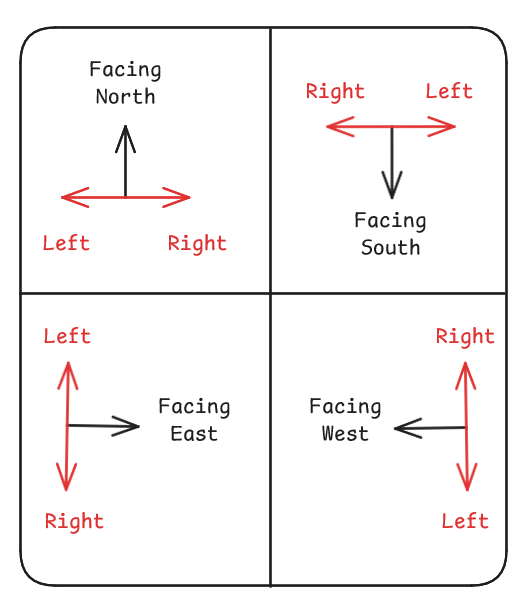
\includegraphics[width=0.4\linewidth]{LRDI/Images/Arrangements_Directions.png}    
\end{figure*}

\begin{NOTE}
    For questions, it is way too much of an effort to create them in latex. I have to see what I can do to do this efficiently later (maybe for next year CAT's attempt)
\end{NOTE}